\section{Аймаг сумдын мэдээлэл авдаг форм}

Уг формыг шаардлагын дагуу алхам алхмаар хөгжүүлснээр React-н анхан шатны туршлагатай болох зорилготой байсан ба цаашид ажилласан төсөл дээр хэрэглэж буй зарим сан болох Material-ui, react-select-н ажиллагааг ойлгох, тодорхой хэмжээнд практик мэдлэгийг цуглуулж чадсан. 

Сурах ур чадвар: 
\begin{itemize}
    \item Асуудлаа тодорхойлж бага багаар шийдвэрлэх чадварт суралцах
    \item Git ашиглах чадвараа нэмэгдүүлэх
    \item Нэг төсөл дээр өөр өөр технологи ашиглах
\end{itemize}

Формын шаардлага: 
\begin{itemize}
    \item Next.js ашигласан байна
    \item Functional component ашиглаж, тухайн component-н дотоод төлвийг ашиглах
    \item Эцэг сонголтыг өөрчлөхөд хүү сонголтуудын утга цэвэрлэгддэг байх
    \item useEffect hook ашиглах
    \item Дараагийн шатанд форм дээрээ Material-ui нэвтрүүлэх
    \item Дараагийн шатанд useReducer ашиглах
    \item Дараагийн шатанд react-select санг нэвтрүүлэх
\end{itemize}

\subsection{useEffect болон useState ашиглан формын мэдээллийг шаардлагын дагуу авах}

Эхний ээлжинд ямар нэгэн загваргүй зөвхөн формын зөв ажиллагаа буюу логик үйлдлүүд дээр анхаарах хэрэгтэй байсан ба хамгийн түрүүнд хийх шаардлагатай зүйл нь аймаг сумдын датаг next.js дээрээ үүсгэсэн api-аасаа авч дэлгэцэнд харуулах байсан юм. 

\begin{lstlisting}[language=Javascript, caption=Next.js дээр бичсэн серверээс датагаа татаж авах, frame=single]
const fetchData = (url) => {
  return axios
    .get(`http://localhost:3000/api/${url}`)
    .then((res) => {
      const results = res.data;
      return results;
    })
    .catch((err) => {
      console.error(err);
    });
};
\end{lstlisting}

Доор харагдаж буй хэсэгт компонентийн логик үйлдлүүд харагдаж байна. useForm() hook ашиглаж select-н утга өөрчлөгдсөн эсэхийг барьж авах, functional component ашиглан state дотор хэрэглэгчийн сонгосон аймаг, сум, хороог хадгална. 

\begin{lstlisting}[language=Javascript, caption=Component-н үндсэн логик үйлдлүүд, frame=single]
export default function Home() {
  const [values, handleChange] = useForm();
  const [data, setData] = useState({
    cities: [],
    districts: [],
    wards: [],
  });

  useEffect(() => {
    fetchData(`cities`)
      .then((res) => {
        setData({ ...data, cities: res });
      })
      .catch((err) => {
        console.error(err);
      });
  }, []);

  const register = (e) => {
    e.preventDefault();
    console.log(values);
  };

  const handleSelect = (id, type) => {
    if (type == "city") {
      fetchData(`cities/${id}`)
        .then((res) => {
          setData({ ...data, districts: res, wards: [] }); //set districts and clear wards data
        })
        .catch((err) => {
          console.error(err);
        });
    } else if (type == "district") {
      //get wards
      fetchData(`cities/${values.city}/${id}`)
        .then((res) => {
          setData({ ...data, wards: res });
        })
        .catch((err) => {
          console.error(err);
        });
    }
  };
  
  ...
\end{lstlisting}

State дотор хэрэглэгчийн сонгосон мэдээллийг зөвөөр хадгалах шаардлагатай байсан. Эхний байдлаар доор харагдаж байгаагаар хадгалсан ч үүссэн асуудлууд нь замбаараагүй, эцэг сонголтыг сонгоход хүү сонголтуудыг цэвэрлэхэд төвөгтэй байв.

\begin{lstlisting}[language=Javascript, caption=Дотоод төлвийн эхний хувилбар, frame=single]
	const [cities, setCities] = useState([]);
  const [districts, setDistricts] = useState([]);
  const [wards, setWards] = useState([]);
  const [selectedCity, setSelectedCity] = useState();
  const [selectedDistrict, setSelectedDistrict] = useState();
  const [selectedWard, setSelectedWard] = useState();
\end{lstlisting}

Иймд state-ээ дараах байдлаар хадгаллаа.

\begin{lstlisting}[language=Javascript, caption=Дотоод төлвийн сайжруулсан хувилбар, frame=single]
	const [data, setData] = useState({
    cities: [],
    districts: [],
    wards: [],
  });
\end{lstlisting}

Эхний шаардлагын дагуу формыг хэрэгжүүлсний дараах вэб дээр харагдах байдал

\begin{figure}
	\centering
	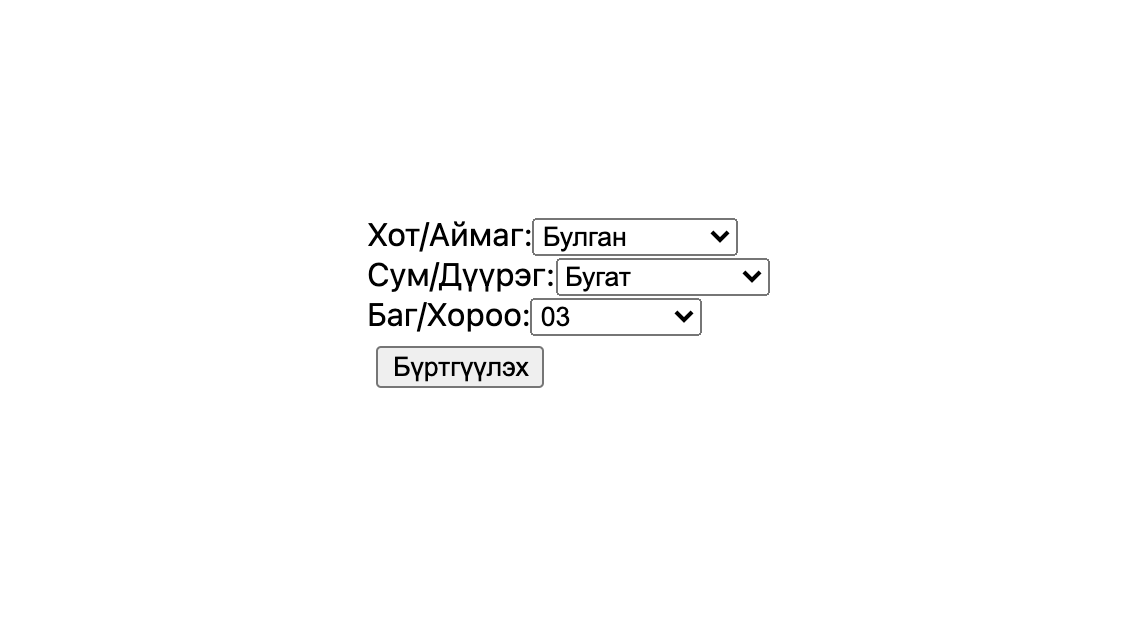
\includegraphics[width=15cm]{images/form-v1.png}
	\caption{Формын эхний хувилбар}
	\label{fig:my_label}
\end{figure}

\pagebreak
\subsection{useState-н оронд useReducer hook ашиглах}

useReducer нь useState hook-н өөр нэг хувилбар бөгөөд өөр дээрээ state болон action гэсэн параметрүүдийг хүлээн авдаг. State нь өгөгдөл хадгалах бол action нь тухайн state дээр ямар үйлдлүүдийг хийх шаардлагатайг хүлээж авдаг. 

Хамгийн түрүүнд Action-ынхаа төрлүүдийг зарлана.

\begin{lstlisting}[language=Javascript, caption=Хийх үйлдлүүдийн төрлийг зарлах, frame=single]
	const SET_CITY = "city";
	const SET_DISTRICT = "district";
	const SET_WARD = "ward";
\end{lstlisting}

Үүний дараа хийх үйлдлүүдээ switch case дотор тодорхойлно. Switch case ашигласнаар олон дахин функц зарлах шаардлагагүйгээр Action-н төрлөөс хамаарч тухайн үйлдлийг ажиллуулна. 

\begin{lstlisting}[language=Javascript, caption=Хийх үйлдлүүдийг тодорхойлох, frame=single]
	const reducer = (state, action) => {
  switch (action.type) {
    case SET_CITY:
      return {
        city: action.index,
        district: null,
        ward: null,
      };
    case SET_DISTRICT:
      return {
        ...state,
        district: action.index,
        ward: null,
      };
    case SET_WARD:
      return {
        ...state,
        ward: action.index,
      };
    default:
      return state;
  }
};
\end{lstlisting}

useReducer ашигласнаар өгсөн шаардлагуудын нэг болох эцэг сонголтыг солиход хүү сонголтууд хоосрох ёстой гэснийг маш хялбар байдлаар шийдэх боломжтой болов. Ердөө тухайн сонголтын доор байгаа state-үүдийн утгыг анхны утгаар солисон.

\begin{lstlisting}[language=Javascript, caption=Хүү сонголтуудыг цэвэрлэх, frame=single]
	...
    case SET_DISTRICT:
      return {
        ...state,
        district: action.index,
        ward: null,
      };
  ...
\end{lstlisting}

Одоо форм дээрээ React-Select санг ашиглаж компонент доторх кодоо бичих шаардлагатай. Энэ хэсэг нь DOM дээр рендерлэгдэнэ. 

\begin{lstlisting}[language=Javascript, caption=React-Select ашигласан байдал, frame=single]
	...  
	<form className={styles.grid} onSubmit={register}>
		<label>
			<p>Country:</p>
			<Select
				value={address.map((i, index) => ({ ...i, index }))[state.city]}
				onChange={(e) => handleChange(e.index, SET_CITY)}
				options={address.map((i, index) => ({ ...i, index }))}
				getOptionLabel={(option) => option.name}
				getOptionValue={(option) => option.index}
				placeholder="Choose"
			/>
		</label>
  ...
\end{lstlisting}
\pagebreak

React-Select болон Material-UI ашигласны дараа формын маань харагдах байдал. Удирдагчийн өгсөн шаардлагуудын дагуу амжилттай хөгжүүлж дууслаа.
\begin{figure}
	\centering
	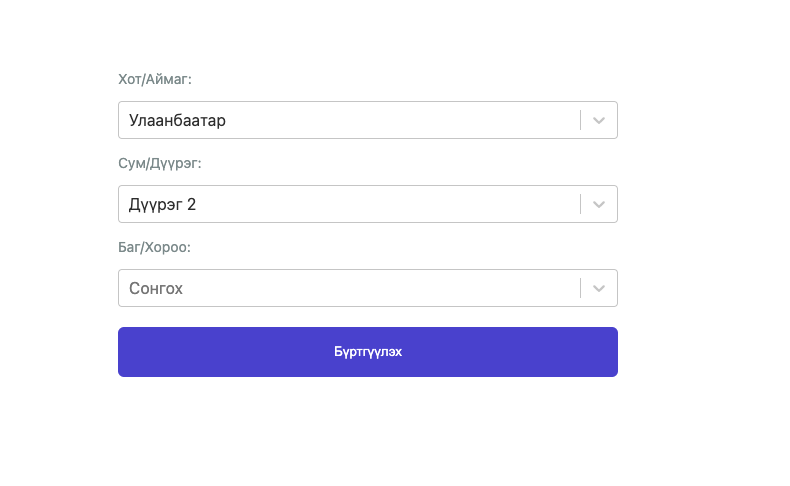
\includegraphics[width=15cm]{images/form.png}
	\caption{Формын эцсийн байдлаар харагдаж буй байдал}
	\label{fig:my_label}
\end{figure}

\section{Toast компонент}

Уг компонентийн гол үүрэг нь Мерчант төсөл дээр ашиглаж буй бүх хүсэлтүүдийн хариуг хэрэглэгч дээр харуулах үүрэгтэй. Мөн хөгжүүлж дууссаны дараа хэрэглэгчийн интерфэйсийн автоматжуулсан тест хийж байж production дээр орох боломжтой.

Сурах ур чадвар: 
\begin{itemize}
    \item State management-н гол ойлголт болох Context-н талаар мэдлэгтэй болно
    \item Өөрийн шаардлагад нийцсэн custom hook бичиж сурах
    \item Хэрхэн бичсэн компонент дээрээ UI автоматжуулсан тест бичих мэдлэг
\end{itemize}

Формын шаардлага: 
\begin{itemize}
    \item Material-UI-н Snackbar ашиглах
    \item Олон Toast зэрэг гаргадаг байх
    \item Toast нь үүсгэх, цэвэрлэх, устгах үйлдлүүдтэй байх
    \item Toast-н цаг дуусахад автоматаар цэвэрлэдэг байх
    \item UI автоматжуулсан тестийг давсан байх
\end{itemize}

\subsection{Context үүсгэх}